\documentclass{article}
\usepackage{gvv-book}
\usepackage{gvv}
\usepackage{amsmath}
\usepackage{amsfonts}
\usepackage{tikz}
\usepackage{setspace}
\usepackage{gensymb}
\usepackage[cmex10]{amsmath}
\usepackage{amsthm}
\usepackage{mathrsfs}
\usepackage{txfonts}
\usepackage{stfloats}
\usepackage{bm}
\usepackage{cite}
\usepackage{cases}
\usepackage{subfig}
\usepackage{longtable}
\usepackage{multirow}
\usepackage{enumitem}
\usepackage{mathtools}
\usepackage{tikz}
\usepackage{circuitikz}
\usepackage{verbatim}
\usepackage[breaklinks=true]{hyperref}
\usepackage{tkz-euclide}
\usepackage{listings}
\usepackage{color}    
\usepackage{array}    
\usepackage{longtable}
\usepackage{calc}     
\usepackage{multirow} 
\usepackage{hhline}   
\usepackage{ifthen}   
\usepackage{lscape}     
\usepackage{chngcntr}
\usepackage{graphicx}
\usepackage{float}
\usepackage{multicol}
\usepackage[a4paper, left = 1.5cm, right = 1.5cm]{geometry}

\begin{document}

\begin{center}
\large
    \textbf{Samyak Gondane-AI25BTECH11029}
\end{center}
\date{}

\section*{Question}
Find the coordinates of the foot of the perpendicular drawn from the point $\vec{A}(-1, 8, 4)$ to the line joining the points $\vec{B}(0, -1, 3)$ and $\vec{C}(2, -3, -1)$. Hence find the image of the point $\vec{A}$ in the line $BC$.

\section*{Solution}

\subsection*{Direction Vector of Line BC}
\begin{align}
\vec{d} = \vec{C} - \vec{B} = 
\myvec{2 \\ -3 \\ -1} - \myvec{0 \\ -1 \\ 3} = \myvec{2 \\ -2 \\ -4}
\end{align}

\subsection*{Parametric Form of Line BC}
\begin{align}
\vec{r}(t) = \vec{B} + t\vec{d} = 
\myvec{
0 \\ -1 \\ 3
}
+ t
\myvec{
2 \\ -2 \\ -4
}
=
\myvec{
2t \\ -1 - 2t \\ 3 - 4t
}
\end{align}

\subsection*{Orthogonality Condition}
\begin{align}
\vec{r}(t) - \vec{A} =
\myvec{2t + 1 \\ -2t - 9 \\ -4t - 1}
\end{align}

$$(\vec{r}(t) - \vec{A}) \cdot \vec{d} = 0$$

\begin{align}
(2t + 1)(2) + (-2t - 9)(-2) + (-4t - 1)(-4) = 0 \\
4t + 2 + 4t + 18 + 16t + 4 = 0 \\
24t + 24 = 0 \Rightarrow t = -1
\end{align}

\subsection*{Foot of Perpendicular}
\begin{align}
\vec{r}(-1) = 
\myvec{0 \\ -1 \\ 3}
+ (-1)
\myvec{2 \\ -2 \\ -4}
=
\myvec{-2 \\ 1 \\ 7}
\end{align}

\subsection*{Image of A in Line BC}
\begin{align}
\vec{A}_{\text{image}} = 2\vec{r}_{\perp} - \vec{A} =
2
\myvec{-2 \\ 1 \\ 7}
-
\myvec{-1 \\ 8 \\ 4}\\
=
\myvec{-4 \\ 2 \\ 14}
+
\myvec{1 \\ -8 \\ -4}
=
\myvec{-3 \\ -6 \\ 10}
\end{align}

\begin{figure}[H]
    \centering
    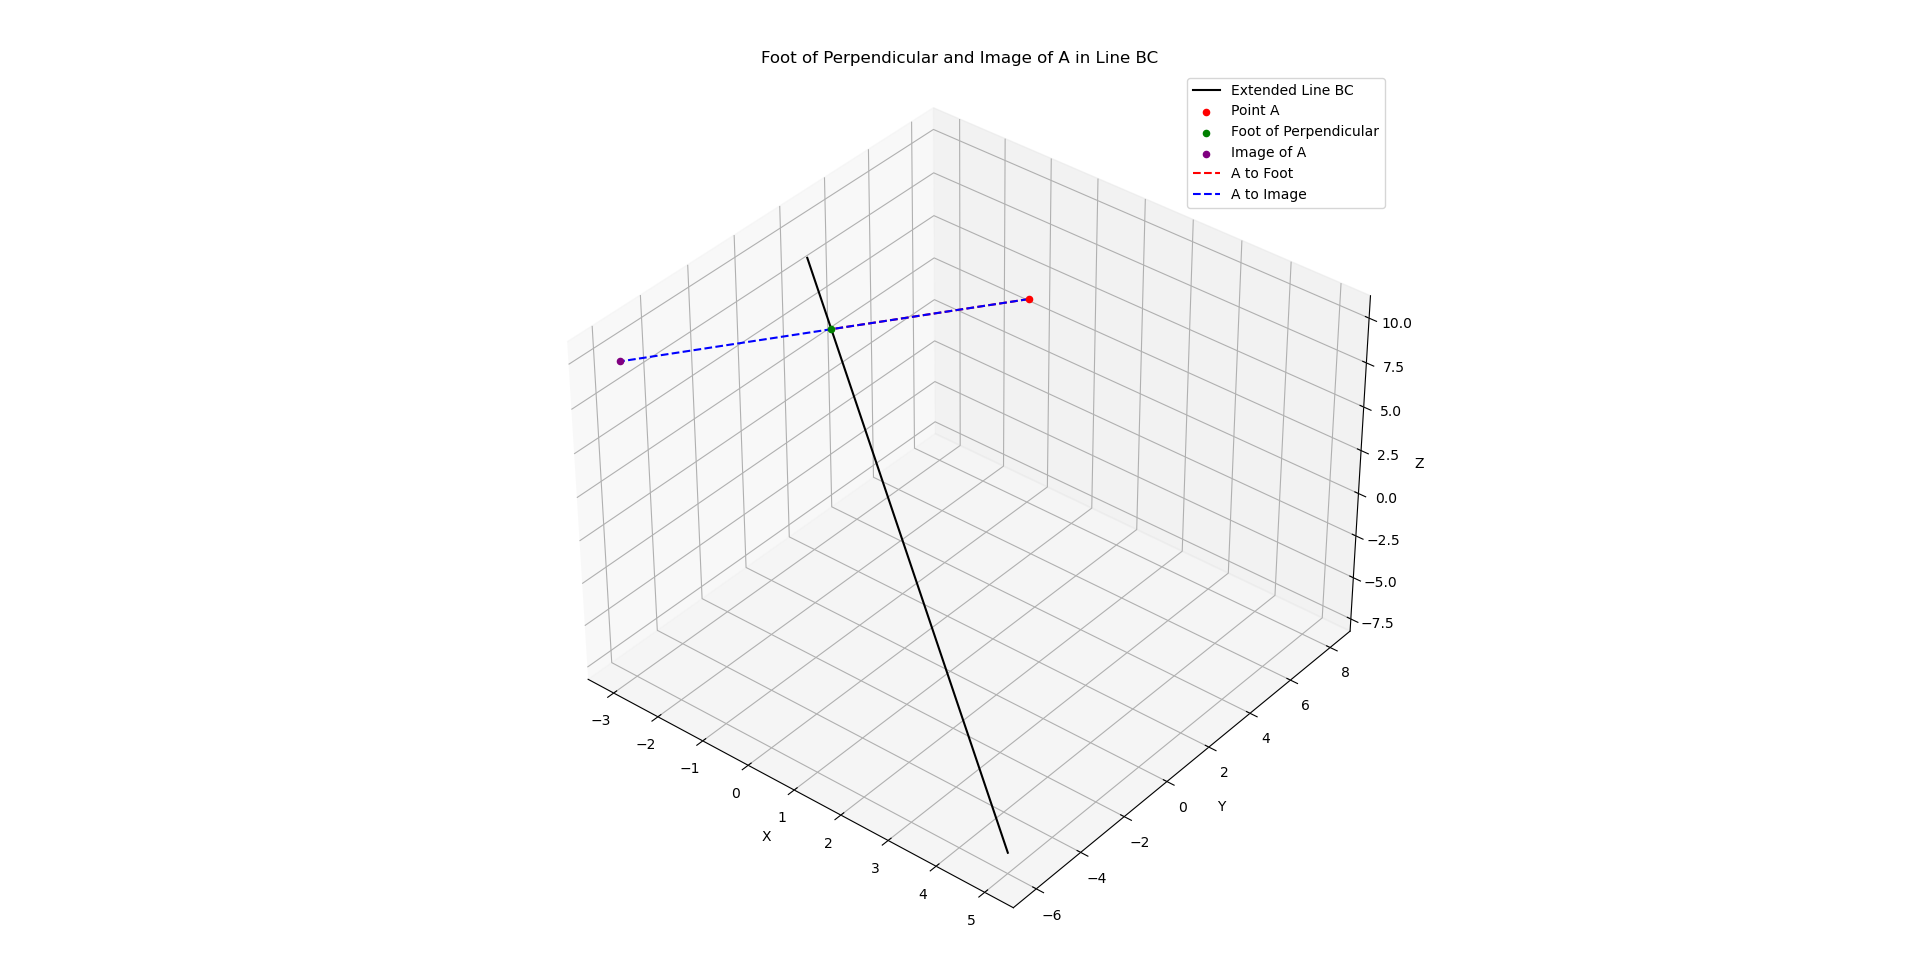
\includegraphics[width=1\linewidth]{./figs/Figure_1.png}
    \caption{}
    \label{fig:fig1}
\end{figure}

\end{document}